\section{User Interface Storyboards}

\subsection{Administrative Functions Use Case: Kobe}
As an administrator, Kobe will need to approve or deny posts as needed and provide explanations for approval or denial (Figure \ref{fig:postmgmt}).  Before approval, Kobe will inspect each post to ensure that the posting follows the website's terms and conditions (Figure \ref{fig:postdetails}).  In addition, he will be able to contact and ban users, delete and edit user posts, and inspect user transaction history.  Priority 1 implementation shall be through MySQL workbench and/or MySQL command line interface.  The following user interface storyboards illustrate a priority 3 implementation for administration through the website.

\begin{figure}[h!]
\caption{Post Management View}
\label{fig:postmgmt}
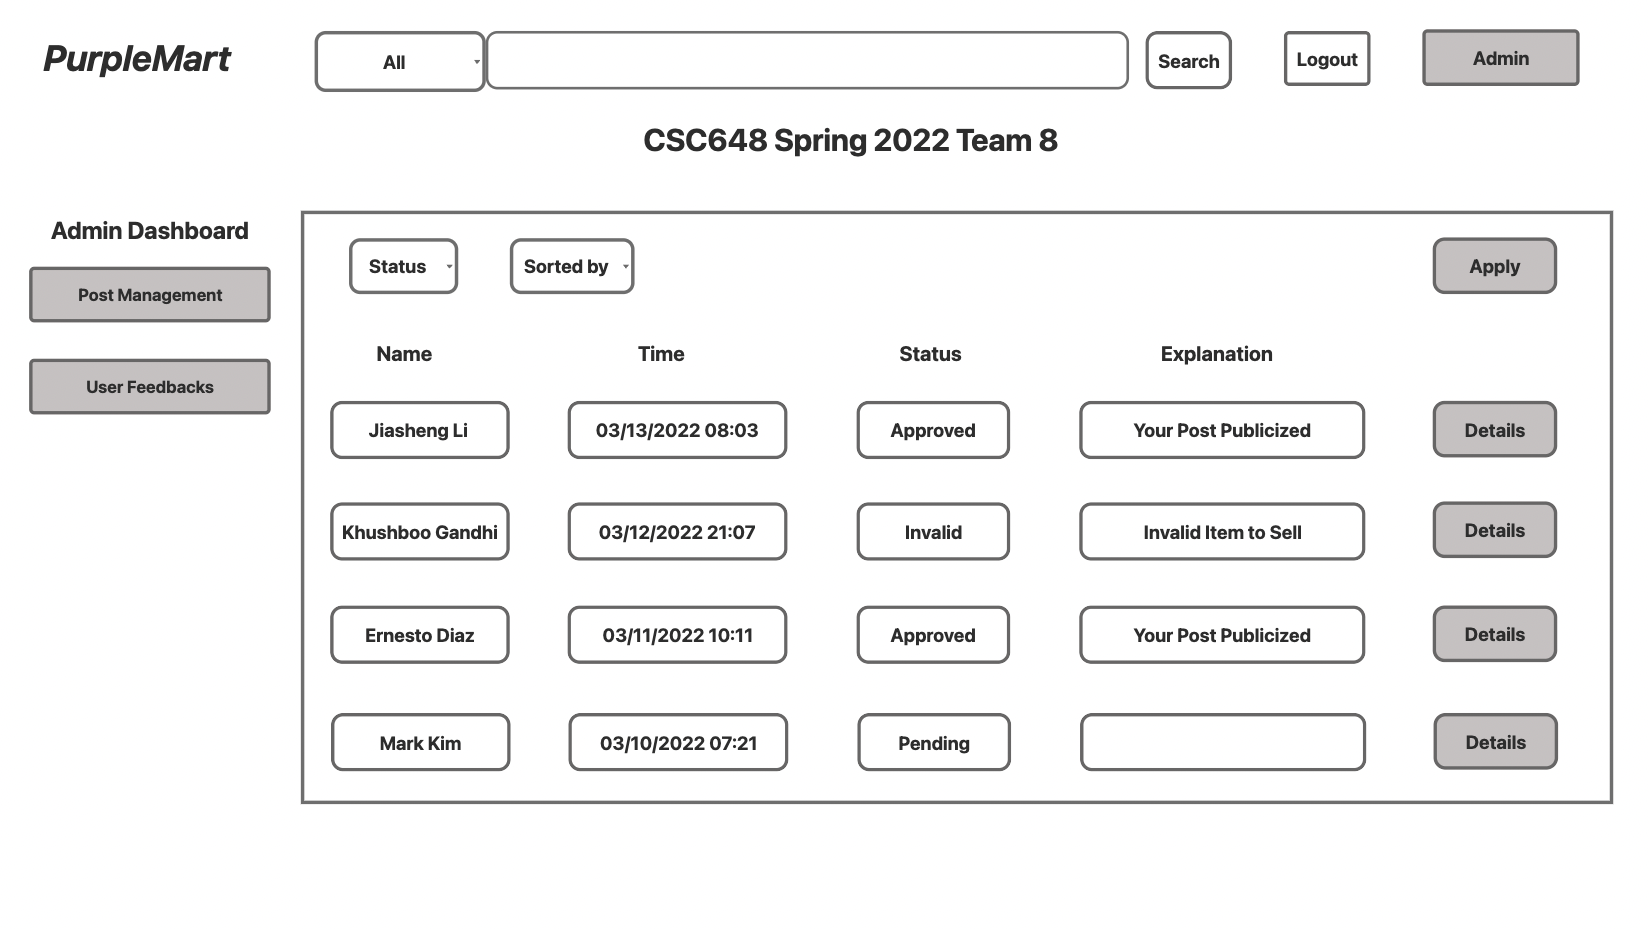
\includegraphics[trim={0 0 0 0}, width=\textwidth]{AdminDashboard_PostManagement}
\end{figure}

\vspace{10mm}

\begin{figure}[h!]
\caption{Post Detail View}
\label{fig:postdetails}
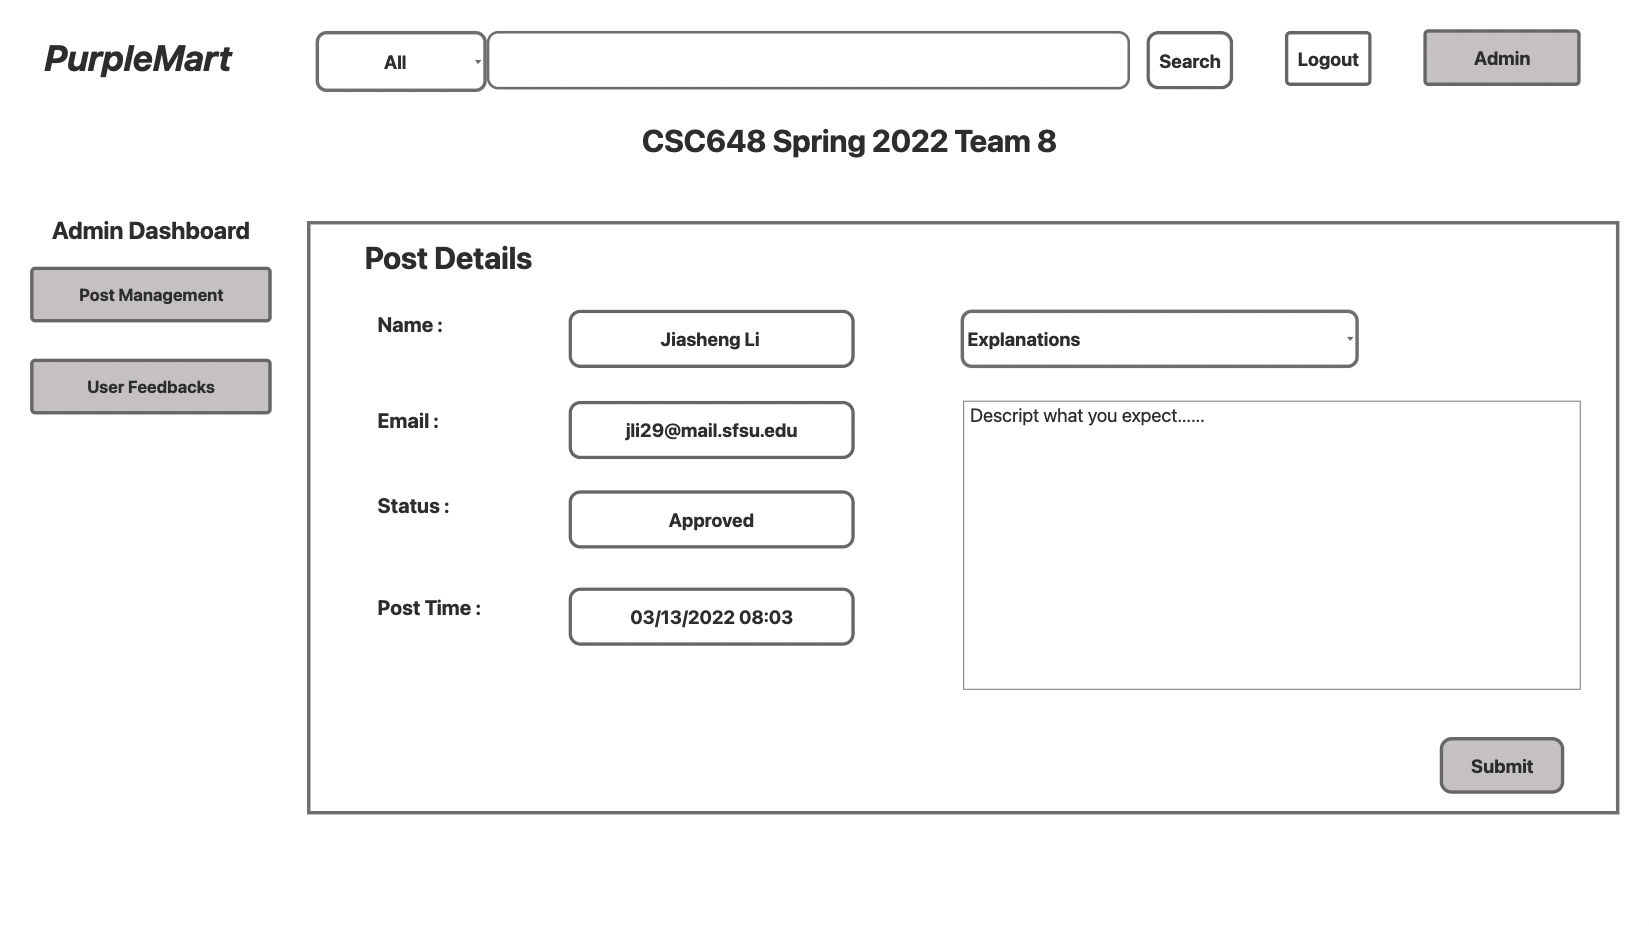
\includegraphics[trim={0 0 0 0}, width=\textwidth]{AdminDashboard_PostDetailEdit}
\end{figure}

\pagebreak
\subsection{Purchase SFSU Apparel Use Case: Claire}
Claire is purchasing SFSU apparel from other users.  Using her laptop, she goes onto PurpleMarket and selects ``SFSU Apparel'' from the categories and browses the available listings (Figure \ref{fig:sfsu}).  Once she finds the swimsuit, she views the item details (Figure \ref{fig:itemc}), then attempts to message the seller for a swimsuit.  The website then informs her that to message a seller, she must first register for a free account or login (Figure \ref{fig:loginc}).  Since she is not signed up, she must register (Figure \ref{fig:regc}).  Once signed up, she is presented with a message page that allows her to message the seller (Figure \ref{fig:msgc}) and the website tells her that her message was successfully sent (Figure \ref{fig:msgconfc}).  Once the transaction is completed, the website prompts her to leave a review.

\vspace{5mm}
\begin{figure}[h!]
\caption{SFSU Apparel Category Search}
\label{fig:sfsu}
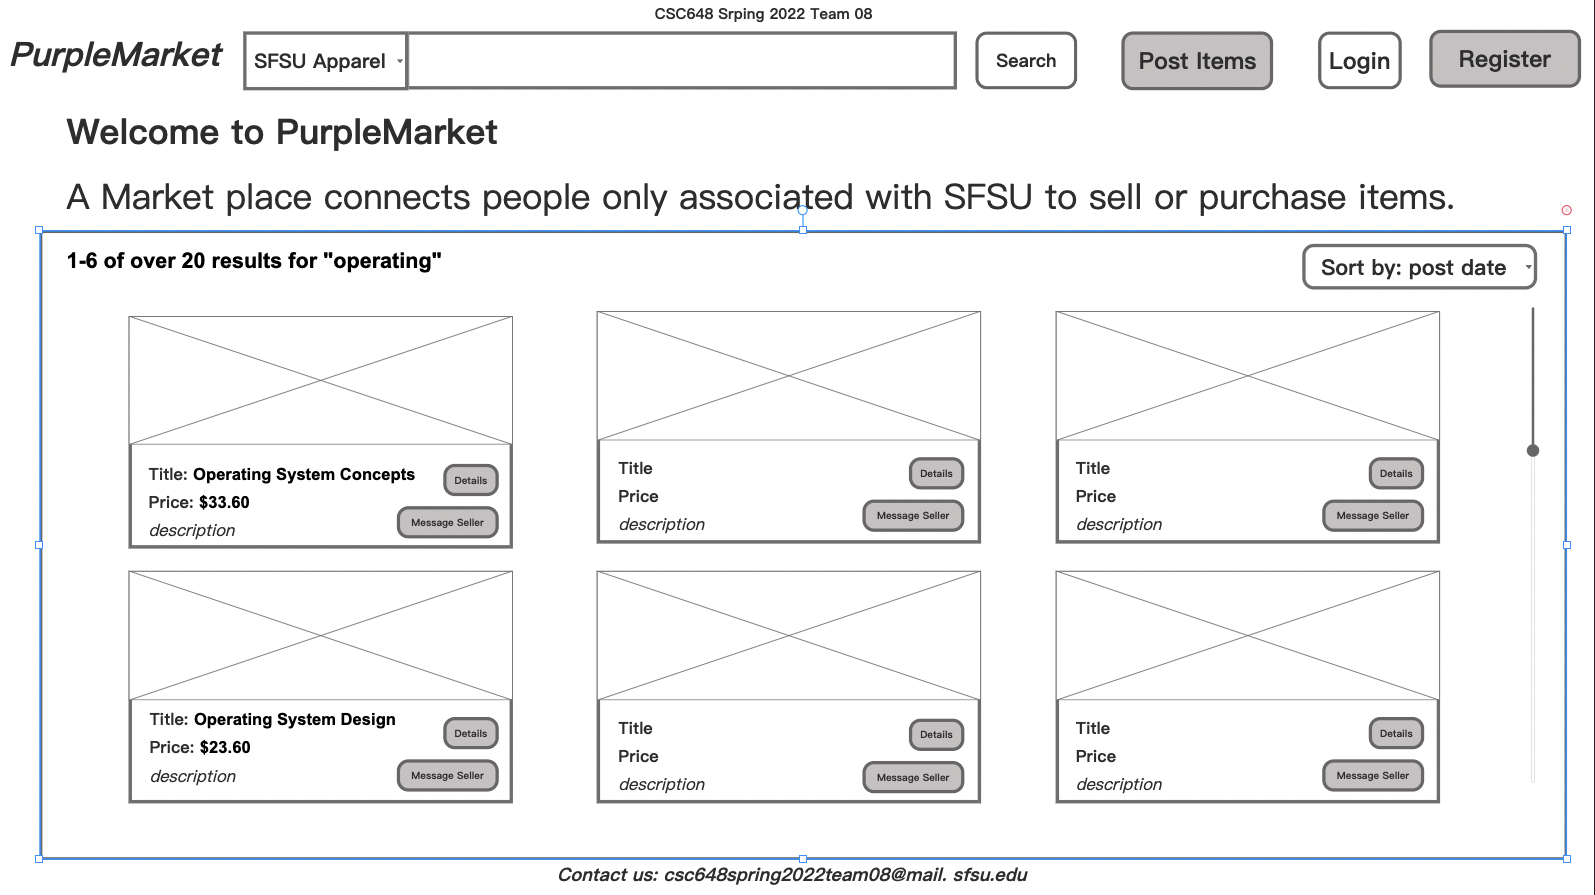
\includegraphics[trim={0 0 0 0}, width=\textwidth]{Search_SFSU}
\end{figure}

\vspace{10mm}

\begin{figure}[h!]
\caption{Item Detail View}
\label{fig:itemc}
\includegraphics[trim={0 -125 0 0}, width=\textwidth]{item}
\end{figure}

\begin{figure}[h!]
\caption{Login View}
\label{fig:loginc}
\includegraphics[trim={0 0 0 0}, width=\textwidth]{login}
\end{figure}

\begin{figure}[h!]
\caption{Registration View}
\label{fig:regc}
\includegraphics[trim={0 -125 0 0}, width=\textwidth]{registration}
\end{figure}

\begin{figure}[h!]
\caption{Message View}
\label{fig:msgc}
\includegraphics[trim={0 0 0 0}, width=\textwidth]{message}
\end{figure}

\begin{figure}[h!]
\caption{Message Confirmation View}
\label{fig:msgconfc}
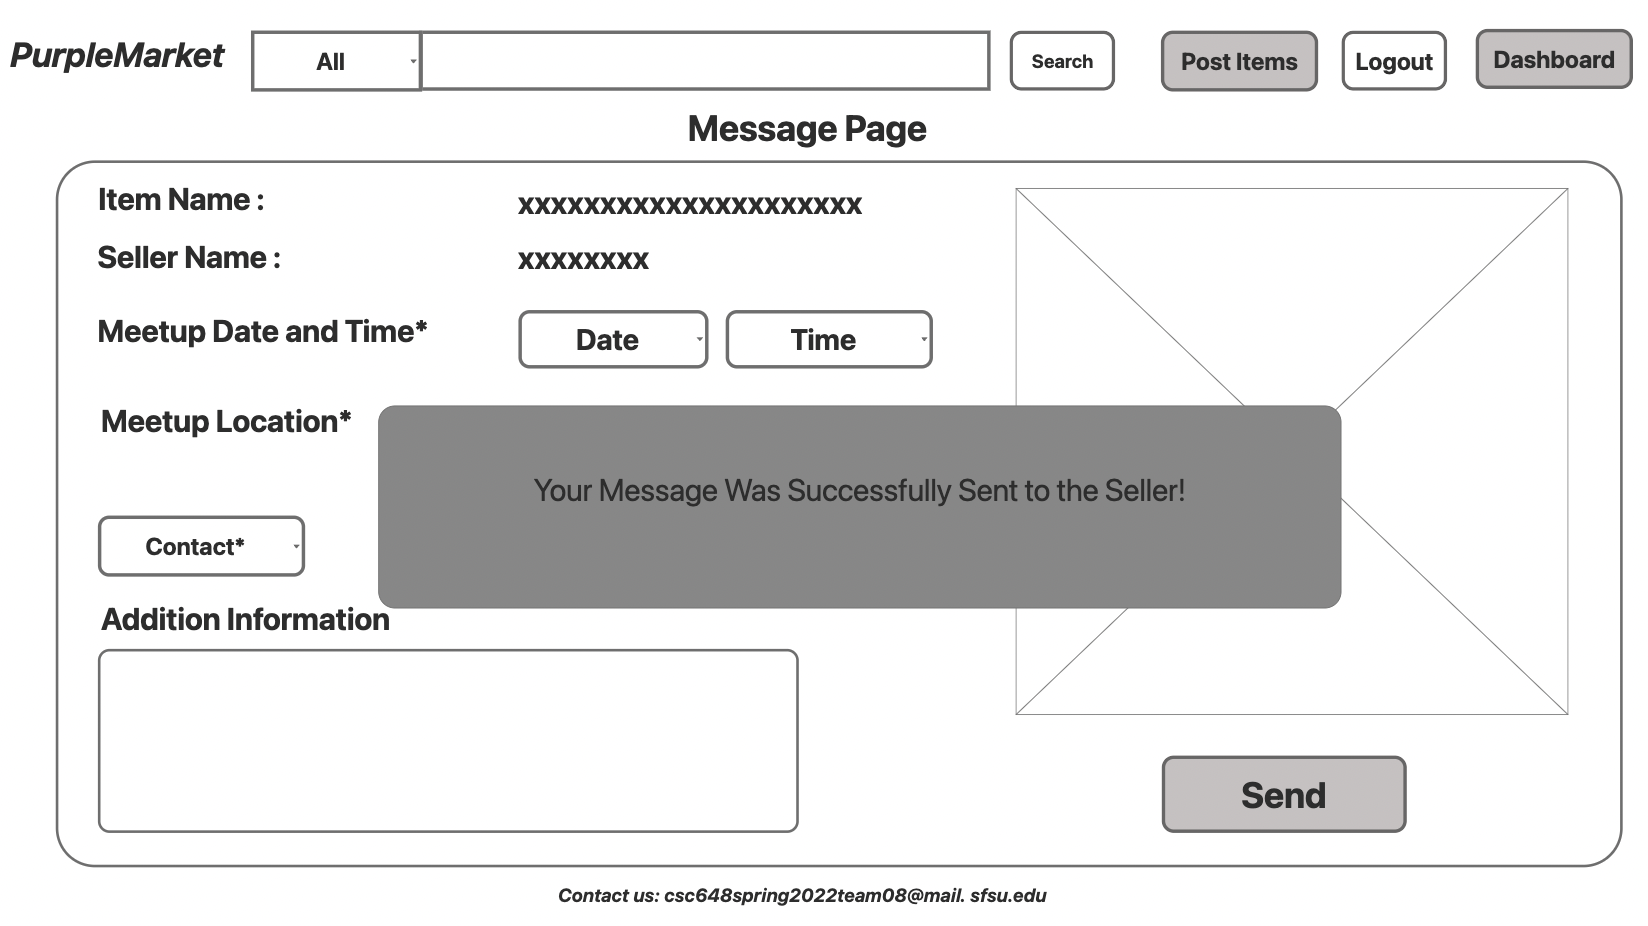
\includegraphics[trim={0 0 0 0}, width=\textwidth]{Message_Confirmation}
\end{figure}

\subsection{Request Items: Anna}
Claire is purchasing SFSU apparel from other users.  Using her laptop, she goes onto PurpleMarket and selects ``SFSU Apparel'' from the categories and browses the available listings (Figure \ref{fig:sfsu}).  Once she finds the swimsuit, she views the item details (Figure \ref{fig:itemc}), then attempts to message the seller for a swimsuit.  The website then informs her that to message a seller, she must first register for a free account or login (Figure \ref{fig:loginc}).  Since she is not signed up, she must register (Figure \ref{fig:regc}).  Once signed up, she is presented with a message page that allows her to message the seller (Figure \ref{fig:msgc}) and the website tells her that her message was successfully sent (Figure \ref{fig:msgconfc}).  Once the transaction is completed, the website prompts her to leave a review.